%-----------------------------------------------
% Dateiname: IntegrationInstallTool.tex
% Autor    : Stefano Kowalke <blueduck@gmx.net>
% Lizenz   : BSD
%-----------------------------------------------
\section{Integration des Prototypen in das Install Tool}
\label{prototype:sec:integrateIntoInstallTool}
Um bereits bei der Installation ein alternatives \gls{dbms} nutzen zu können, mußte der Prototyp breits über das \textit{Install Tool} installierbar sein, was Anpassungen an dem \textit{Install Tool} und TYPO3 CMS zur Folge hatte.

Wie in Kapitel~\ref{prototype:subsec:installTYPO3} zu sehen war, besteht das \textit{Install Tool} aus fünf Schritten, die durch die Klassen im Ordner \pdf{typo3/sysext/install/Classes/Controller/Action/Step} bereitgestellt werden. Der StepController \pdf{typo3/sysext/install/Classes/Controller/Action/StepController} iteriert bei jedem Reload des Installtools über alle Schritte und prüft ob der jeweils aktuelle Schritt bereits ausgeführt wurde oder noch ausgeführt werden muß. Er erkennt dies an Bedingungen, die von jedem Schritt definiert werden. Sind alle Bedingungen erfüllt, findet ein Redirekt auf den nächsten Schritt statt.

Die Ausgabe der Schritte erfolgt über verschiedene HTML-Template Dateien, die in der TYPO3 eigenen Template-Sprache \textit{Fluid} verfasst sind. Das \textit{Install Tool} setzt hier das \gls{mvc}-Pattern ein, um die Geschäftslogik von der Präsentation zu trennen.

Die HTML-Templates unterteilen sich in \textit{Layouts}, \textit{Templates} und \textit{Partials}, die in den jeweilig gleichnamigen Verzeichnissen in \pdf{typo3/sysext/install/Resources/Privat/} zu finden sind.

\begin{itemize}
	\item Ein Template beschreibt die grundlegende Struktur einer Seite. Typischerweise befindet sich darin der Seitenkopf und -fuß.
	\item Die Struktur einer einzelnen Seite wird von einem Template festgelegt.
	\item Partials stellen wiederkehrende Elemente dar. Sie können in Layout- und Templatedateien eingebunden werden. Die Schaltfläche \textit{I do not use MySQL} aus Abbildung~\ref{fig:installTYPO3LegacyStepTwo} in Kapitel~\ref{prototype:subsec:TwoInsertDatabaseData} ist ein Beispiel für ein Partials.
\end{itemize}


Im folgenden werden die vorgenommenen Änderungen im Detail beschrieben.

\begin{itemize}
\item Eine von Composer erstellte \textit{Autoload}-Datei, wurde in die Datei \phpinline{\TYPO3\CMS\Core\Core\Bootstrap} eingebunden. Somit können die von Doctrine DBAL zur Verfügung gestellten Klassen geladen werden. Siehe~\ref{lst:composerAutoload}
\item In \pdf{typo3/sysext/install/Resources/Private/Partials/Action/Step/DatabaseConnect/} wurden die Partials \pdf{LoadDoctrineDbal.html} und \pdf{UnloadDoctrineDbal.html} zur De- und Installation des Prototypen und das Partial \pdf{DoctrineDbalDriverSelection.html} für die Auswahl des Datenbanktreibers erstellt
\item diese wurden dem zweiten Schritt \pdf{typo3/sysext/install/Resources/Private/Partials/Action/Step/DatabaseConnect.html} hinzugefügt. Die Variable \texttt{isDoctrineEnabled} enthält den Installationsstatus des Prototypen. Abhängig von ihr wird entweder die Schaltfläche zur Installation des Prototypen oder das Auswahlfeld für die Datenbanktreiber und die Schaltfläche zur Deinstallation des Prototypen anzeigt.
\item damit die Variable einen Wert enthält, wurde diese von der \textit{Action} aus \phpinline{\TYPO3\CMS\Install\Controller\Action\Step\DatabaseConnect.php} definiert und an die View übergeben.
\item in \phpinline{\TYPO3\CMS\Install\Controller\Action\Step\DatabaseConnect.php} wurden Methoden erstellt, die die installierten PDO-Extensions des Systems abfragen und an die View übergeben
\item Zur Vermeidung leere Werte in der Konfigurationsdatei, wurden die Prüfungen der Benutzereingaben von \phpinline{isset()} auf \phpinline{!empty()} geändert.
\item Das Eingabeformular für die Datenbankverbindungsinformationen wurde angepasst. Es wurde ein Feld für das \textit{Charset} der Datenbank hinzugefügt und das Feld für die Datenbank entfernt, da sie im einem anderen Schritt über ein Auswahlfeld festgelegt wird.
\item Damit die eingebenen Daten weiterverarbeitet werden konnten, wurden diese in den entsprechenden PHP-Klassen ergänzt. Listing~\ref{lst:saveDoctrineDriverToLocalConf} zeigt das die Abfrage und Speicherung des ausgewählten Datenbanktreibers durch \phpinline{\TYPO3\CMS\Install\Controller\Action\Step\DatabaseConnect.php} in der Konfigurationsdatei. Siehe~\ref{lst:saveDoctrineDriverToLocalConf}
\item Externe Abhängigkeiten werden vom Package Manager in \pdf{thesis.dev/http/Packages/Library} erwartet. Aus diesem Grund mußte der Ordner \pdf{thesis.dev/http/typo3conf/ext/doctrine\_dbal/vendor/doctrine} nach \pdf{thesis.dev/http/Packages/Library/} kopiert werden.\footnote{Composer Konfigurationsdateien werden seit TYPO3 CMS 6.2 analysiert. Aus den definierten Abhängigkeiten und den (System)-Extensions wird vom Package Mananger ein Graph von Abhängigkeiten aufgebaut welcher in \pdf{thesis.dev/http/typo3conf/PackagesStates.php} gespeichert wird. Diese Datei wird bei der Installation erstellt und stetig aktualisiert. Da diese Funktionalität relativ neu ist, mußte diese Datei bei der Installation des Prototypen manuell angepasst werden.}
\end{itemize}

\begin{listing}[H]
\begin{phpcode}
public function initializeClassLoader() {
	/** Composer loader */
	require_once PATH_typo3conf . 'ext/doctrine_dbal/vendor/autoload.php';

	$classLoader = new ClassLoader($this->applicationContext);
	...
}
\end{phpcode}
\caption{Einbinden des vom Composer erstellten Autoloaders}
\label{lst:composerAutoload}
\end{listing}

\begin{listing}
\begin{phpcode}
elseif (isset($postValues['setDoctrineDriver'])) {
  $localConfigurationPathValuePairs['DB/driver'] = $postValues['setDoctrineDriver'];
  $configurationManager->setLocalConfigurationValuesByPathValuePairs($localConfigurationPathValuePairs);
}
\end{phpcode}
\caption{Speicherung des Datenbanktreibers in der LocalConfiguration.php [DatabaseConnect.php]}
\label{lst:saveDoctrineDriverToLocalConf}
\end{listing}

%\begin{htmlcode}
%<f:if condition="{isDoctrineEnabled}">
	%<f:then>
		%<f:render partial="Action/Step/DatabaseConnect/DoctrineDbalDriverSelection" arguments="{_all}" />
		%<f:if condition="{selectedDoctrineDriver}">
			%<f:render partial="Action/Step/DatabaseConnect/ConnectDetails" arguments="{_all}" />
		%</f:if>
		%<f:render partial="Action/Step/DatabaseConnect/UnloadDoctrineDbal" arguments="{_all}" />
	%</f:then>

	%<f:else>
		%<f:render partial="Action/Step/DatabaseConnect/ConnectDetails" arguments="{_all}" />
		%<f:render partial="Action/Step/DatabaseConnect/LoadDoctrineDbal" arguments="{_all}" />
		%<f:render partial="Action/Step/DatabaseConnect/LoadDbal" arguments="{_all}" />
	%</f:else>
%</f:if>
%\end{htmlcode}

%\begin{listing}
%\begin{phpcode}
%$isDbalEnabled =
  %\TYPO3\CMS\Core\Utility\ExtensionManagementUtility::isLoaded('doctrine_dbal');

%$this->view
  %->assign('isDoctrineEnabled', $isDoctrineEnabled)
  %->assign('username', $this->getConfiguredUsername())
  %->assign('password', $this->getConfiguredPassword())
  %->assign('host', $this->getConfiguredHost())
  %->assign('port', $this->getConfiguredOrDefaultPort())
  %->assign('database', $GLOBALS['TYPO3_CONF_VARS']['DB']['database'] ?: '')
  %->assign('socket', $GLOBALS['TYPO3_CONF_VARS']['DB']['socket'] ?: '');
%\end{phpcode}
%\caption{Zuweisung von in PHP definierten Variablen an die View}
%\end{listing}

Im Folgenden wird die Installation von TYPO3 CMS zusammen mit dem Prototypen erläutert.

\subsection{Schritt 1 - Systemcheck}
	Der erste Schritt entspricht dem aus Kapitel~\ref{prototype:subsec:OneSystemcheck}

\subsection{Schritt 2 - Eingabe der Datenbankdaten}
	Im zweiten Schritt (Abb.:~\ref{fig:installTYPO3DoctrineStepTwoA}) wird nun durch Betätigung der Schaltfläche \textit{I want use Doctrine DBAL} Doctrine DBAL installiert, worauf eine entsprechende Meldung darüber zusammen mit dem Auswahlfeld für den Datenbanktreiber erscheint. Nach der Auswahl des Treibers werden die Inputfelder eingeblendet. Da die verschiedenen \gls{dbms} unterschiedliche Daten für den Aufbau einer Verbindung zur Datenbank benötigen, ist die Anzahl und Art der Felder von dem ausgewählten Treiber abhängig. Der Codeteil ist in der Datei \pdf{typo3/sysext/install/Classes/Controller/Action/Step/DatabaseConnect.php} ab Zeile 556 zu finden. Abbildung~\ref{fig:installTYPO3DoctrineStepTwoB} zeigt die  Felder für MySQL.

\subsection{Schritt 3 - Auswahl der Datenbank}
	Nachdem die Verbindungsdaten eingegeben wurden, versucht TYPO3 CMS eine Verbinung zum \gls{dbms} zu etablieren. Gelingt dies, werden alle verfügbaren Datenbanken abgefragt und aufgelistet (Abb.:~\ref{fig:installTYPO3LegacyStepThree}). Über die Auswahl kann eine leere Datenbank festgelegt werden. Alternativ kann über das Inputfeld eine zu erstellende Datenbank angegeben werden. Mit dem Absenden des Formulars werden die Basistabellen in der Datenbank angelegt.
[SCHEMA BESCHREIBEN]

\subsection{Schritt 4 - Einrichten eines TYPO3 Administrators}
	Der Schritt entspricht dem aus Kapitel~\ref{prototype:subsec:FourCreateAdmin}
\subsection{Schritt 5 - Abschluß der Installation}
	Der Schritt entspricht dem aus Kapitel~\ref{prototype:subsec:FiveDone}


	\begin{figure}[H]
		\begin{subfigure}[b]{0.5\textwidth}
			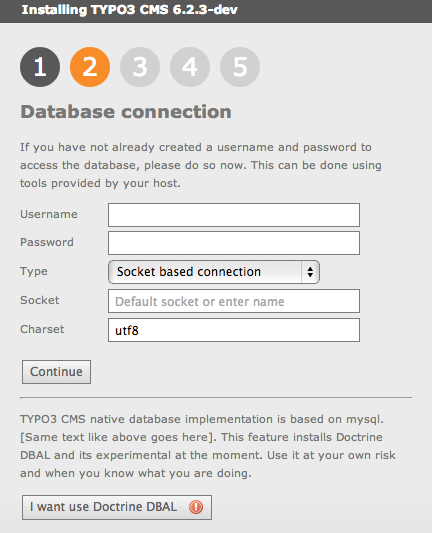
\includegraphics[width=\textwidth]{InstallingTYPO3/DoctrineDBAL/02-DatabaseConnection.png}
			\caption{Installation TYPO3 CMS mit Prototyp - Schritt 2a}
			\label{fig:installTYPO3DoctrineStepTwoA}
		\end{subfigure}%
		~ %add desired spacing between images, e. g. ~, \quad, \qquad, \hfill etc.
	%(or a blank line to force the subfigure onto a new line)
		\begin{subfigure}[b]{0.5\textwidth}
			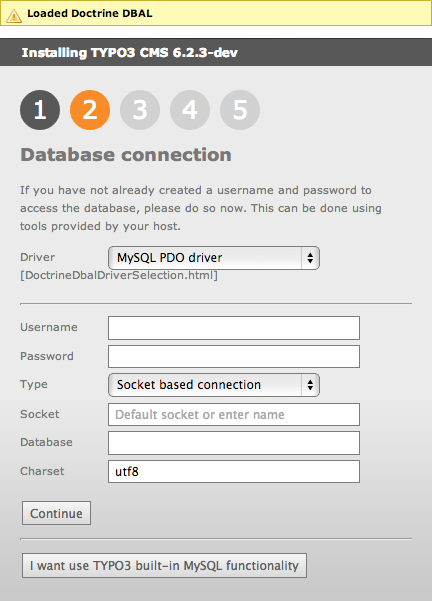
\includegraphics[width=\textwidth]{InstallingTYPO3/DoctrineDBAL/03-DatabaseConnectionDoctrineLoaded.png}
			\caption{Installation TYPO3 CMS mit Prototyp - Schritt 2b}
			\label{fig:installTYPO3DoctrineStepTwoB}
		\end{subfigure}
		~ %add desired spacing between images, e. g. ~, \quad, \qquad, \hfill etc.
	%(or a blank line to force the subfigure onto a new line)
		\caption{Installation von TYPO3 CMS mit den Prototyp}
		\label{fig:installationOfTYPO3}
	\end{figure}



Zur Überprüfung ob TYPO3 CMS tatsächlich den Prototypen nutzt, wurde in der \gls{ide} ein Debug-Breakpoint in die Klasse \phpinline{Konafets\DoctrineDbal\Persistence\Legacy\DatabaseConnection} innerhalb der \phpinline{connectDB} gesetzt, an dem die \gls{ide} die Ausfühung von TYPO3 CMS anhielt als er erreicht wurde.


\subsection{Doctrines Schemarepräsentation}

\subsection{Implementation einer fluenten Query-Language}

